{
\usebackgroundtemplate{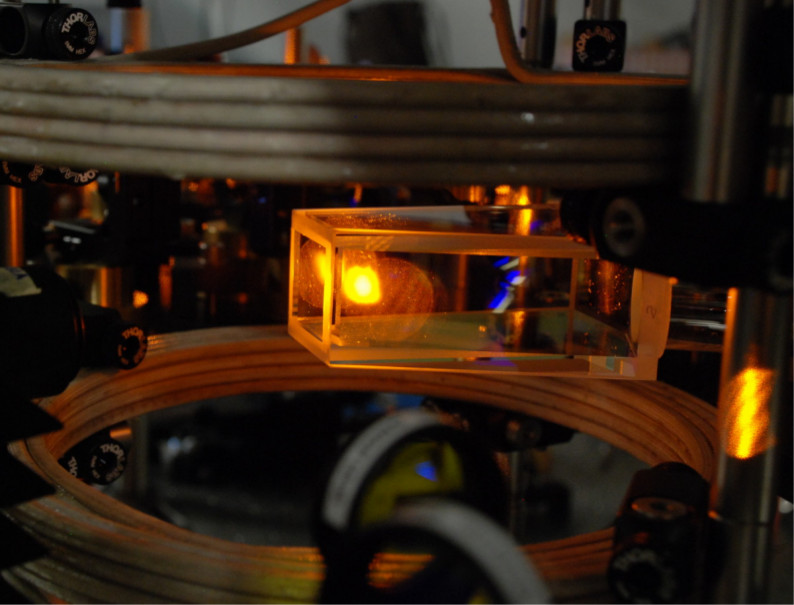
\includegraphics[width=\paperwidth]{Figures/MOT-picture.jpg}}
\begin{frame}[c,plain]

%\vspace{18em}
%
%\only<2>{
%\begin{flushright}
%\textcolor{white}{
%Easy to implement \& highly flexible\\
%\vspace{0.5em}
%Well defined interfaces, defects\\
%\vspace{0.5em}
%On-site properties control (resonance, loss) \\
%\vspace{0.5em}
%LDOS measurement \& direct imaging of the wavefunctions \\
%\vspace{0.5em}
%Transport measurement
%}
%\end{flushright}
%}

%\only<1->{
\btVFill{
\begin{flushright}
\textcolor{white}{\textbf{Our experimental setup to create \textcolor{bellblue}{sodium} BECs}}
\end{flushright}
}
%}

\end{frame}
}
